\documentclass{article}
\usepackage{tikz}
\usepackage{amsmath}

\begin{document}

\begin{figure}
\centering
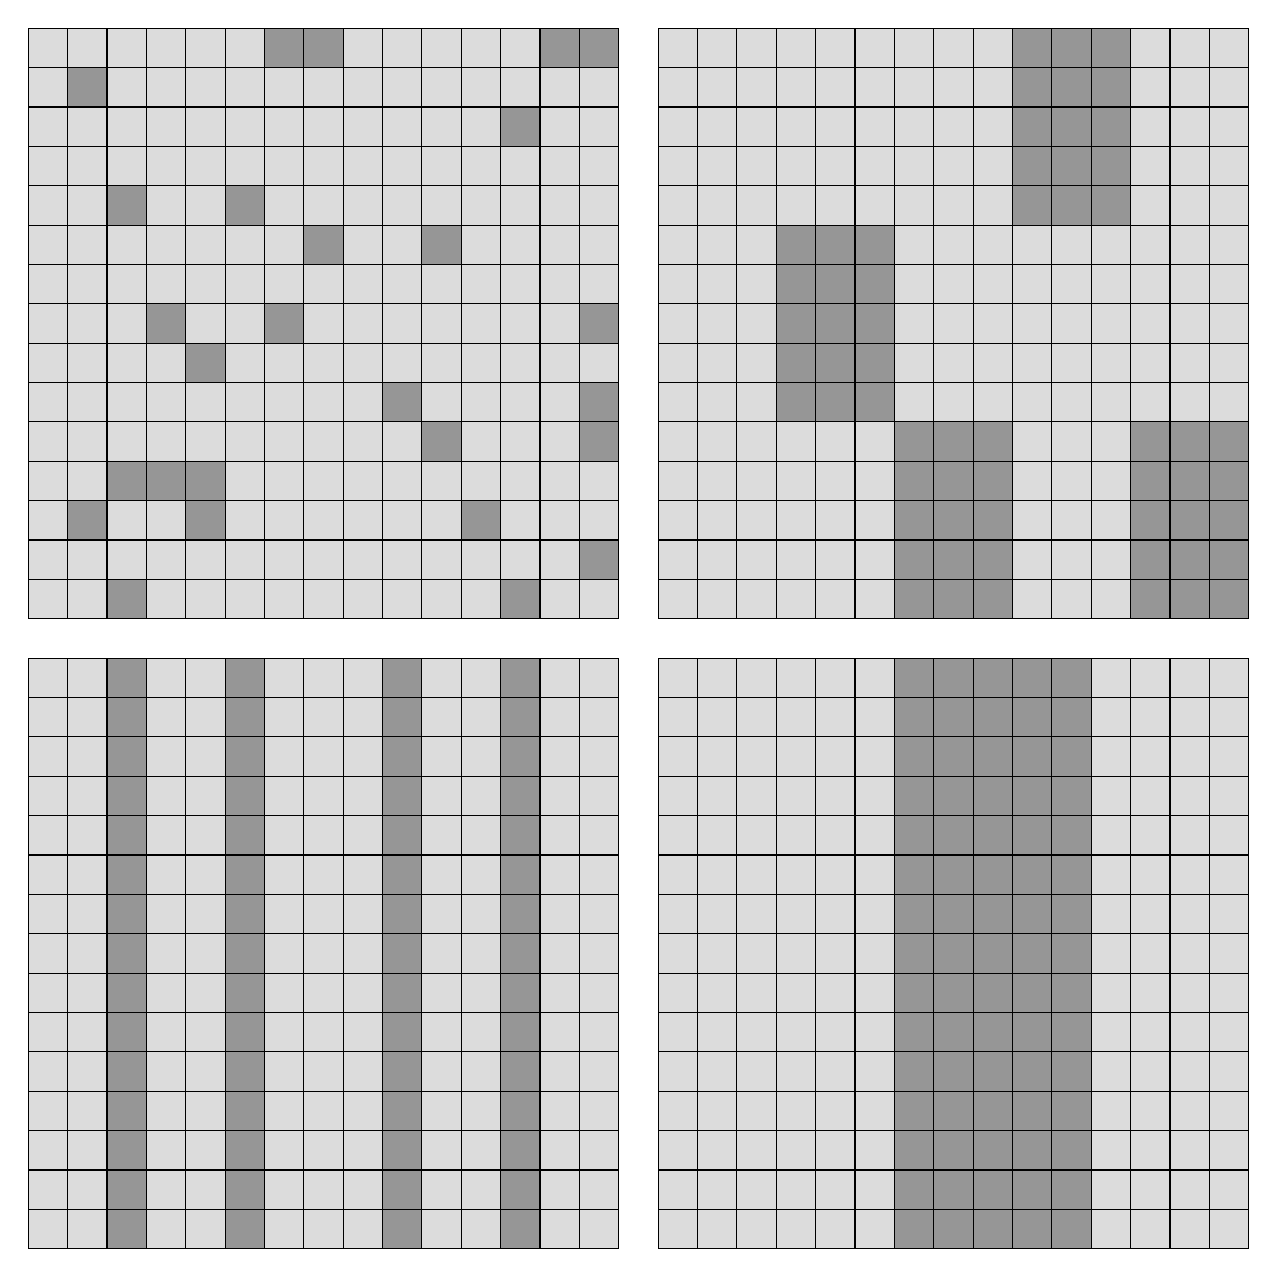
\begin{tikzpicture}[scale=0.5]
% Define colors
\definecolor{lightgray}{RGB}{220,220,220}
\definecolor{darkgray}{RGB}{150,150,150}

% Random Sparsity
\begin{scope}
    % Grid and title
    \node[anchor=south] at (7.5, 13) {\textbf{Random Sparsity}};
    
    % Draw the grid
    \foreach \i in {0,...,14} {
        \foreach \j in {0,...,14} {
            \pgfmathsetmacro{\randnum}{rnd}
            \ifnum\i=0\ifnum\j=0\def\fillcolor{lightgray}\else\def\fillcolor{lightgray}\fi\else
            \pgfmathsetmacro{\fillcolor}{ifthenelse(\randnum < 0.85, "lightgray", "darkgray")}
            \fi
            \fill[\fillcolor] (\i,\j) rectangle +(1,1);
            \draw (\i,\j) rectangle +(1,1);
        }
    }
\end{scope}

% Block Random Sparsity
\begin{scope}[xshift=16cm]
    % Grid and title
    \node[anchor=south] at (7.5, 13) {\textbf{Block Random Sparsity}};
    
    % Draw the grid
    \foreach \i in {0,...,14} {
        \foreach \j in {0,...,14} {
            \pgfmathsetmacro{\randblock}{int(mod(\i,3))}
            \pgfmathsetmacro{\randrow}{int(mod(\j,5))}
            \pgfmathsetmacro{\randnum}{rnd}
            
            % Create block pattern
            \pgfmathsetmacro{\isblock}{ifthenelse(\randnum < 0.7, 1, 0)}
            
            % If it's a block, fill all cells in the block
            \pgfmathsetmacro{\fillcolor}{ifthenelse(
                (int(\i/3) == 1 && int(\j/5) == 1) || 
                (int(\i/3) == 3 && int(\j/5) == 2) ||
                (int(\i/3) == 2 && int(\j/5) == 0) ||
                (int(\i/3) == 4 && int(\j/5) == 0), 
                "darkgray", "lightgray")}
            
            \fill[\fillcolor] (\i,\j) rectangle +(1,1);
            \draw (\i,\j) rectangle +(1,1);
        }
    }
\end{scope}

% Random Column Sparsity
\begin{scope}[yshift=-16cm]
    % Grid and title
    \node[anchor=south] at (7.5, 13) {\textbf{Random Column Sparsity}};
    
    % Draw the grid
    \foreach \i in {0,...,14} {
        % Determine if column is sparse
        \pgfmathsetmacro{\randnum}{rnd}
        \pgfmathsetmacro{\isColumnSparse}{ifthenelse(\randnum < 0.7, 1, 0)}
        
        \foreach \j in {0,...,14} {
            % If column is sparse, make it dark
            \pgfmathsetmacro{\fillcolor}{ifthenelse(
                \i == 2 || \i == 5 || \i == 9 || \i == 12, 
                "darkgray", "lightgray")}
            
            \fill[\fillcolor] (\i,\j) rectangle +(1,1);
            \draw (\i,\j) rectangle +(1,1);
        }
    }
\end{scope}

% Block Random Column Sparsity
\begin{scope}[xshift=16cm, yshift=-16cm]
    % Grid and title
    \node[anchor=south] at (7.5, 13) {\textbf{Block Random Column Sparsity}};
    
    % Draw the grid
    \foreach \i in {0,...,14} {
        \foreach \j in {0,...,14} {
            % Create block column pattern
            \pgfmathsetmacro{\fillcolor}{ifthenelse(
                (\i >= 6 && \i <= 10), 
                "darkgray", "lightgray")}
            
            \fill[\fillcolor] (\i,\j) rectangle +(1,1);
            \draw (\i,\j) rectangle +(1,1);
        }
    }
\end{scope}

\end{tikzpicture}
\caption{Types of sparsity. In random sparsity, any bit may be non-zero. Block-random sparsity assumes aligned, contiguous regions of each row are sparse or not sparse. The degree of block-random sparsity may be lower than the fraction of sparsity when 0s are not fully aligned. We also show random column and random block column sparsity. Block column patterns arise in Deja Vu~\cite{liu2023deja}.}
\end{figure}

\end{document}